\section{Use cases}
\label{sec:usecases}

\eat{Evolving graph analysis algorithms are numerous, including structural
and spatio-temporal graph mining that looks for patterns in space and
time and analytics that investigate the evolution of some property of
the graph over time.}

An interaction network is one typical kind of an evolving graph.  It
represents people as nodes, and interactions between them such as
messages, conversations, and endorsements, as edges.  Information
describing people and their interactions is represented by node and
edge attributes.  One easily accessible interaction network is the
wiki-talk
dataset\footnote{\url{http://dx.doi.org/10.5281/zenodo.49561}},
containing messaging events among Wikipedia contributors over a
13-year period.  Information available about the users includes their
username, group membership, and the number of Wikipedia edits they
made.  Messaging events occur when users post on each other's talk
pages.

We now present common analysis tasks and show how they can be
expressed in \tga. We are primarily interested in analyses of the {\em
  evolution} of the phenomena the graph represents in the form of
queries\eat{ posed by the user}.  The examples were selected for their
breadth, based on the analysis of the related work.

\subsection{Node Influence Over Time}

In an interaction graph, node centrality is a measure of how important
or influential nodes are in the graph.  \eat{Over a dozen different
centrality measures exist, providing indicators of how much
information ``flows'' through the node or how the node contributes
to the overall cohesiveness of the network.  }Node importance
fluctuates over time.  To see whether the wiki-talk graph has
high-importance nodes, and how stable node importance is over
time during a particular period of interest, we can:

%\begin{itemize}%[noitemsep,topsep=0pt]
%\item Look at a subset of the graph that corresponds to the period of interest.
%\item Compute an importance measure, such as in-degree, for each node and for each
%point in time.
%\item Calculate the coefficient of variation per node.
%\end{itemize}
%
%This example demonstrates a need to select a subset of the data
%corresponding to the period of interest, compute in-/out-degree for
%each node at each point in time, and compute a single measure across
%time for each node.  Computation of degree is a simple example of a
%non-temporal {\em aggregation} operation as defined by the taxonomy of
%Wood~\cite{Wood2012}.  Aggregation computes a value for each node
%based on its neighbors and can be used for a wide variety of analyses.

\begin{figure}
\centering
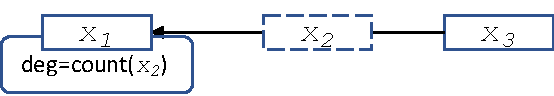
\includegraphics[width=2.5in]{figs/degrees.pdf}
\vspace{-0.2cm}
\caption{Temporal navigational graph pattern $p_1$ to compute node degrees.}
\label{fig:degrees}
\vspace{-0.2cm}
\end{figure}

\begin{enumerate}[itemindent=\dimexpr\labelwidth+\labelsep\relax,leftmargin=0pt]
\item Select a subset of the data representing the 5 years of
  interest, using \insql{trim}:  $\ttt_1 = \slice{[2010,2015)}{wikitalk}$

\item Compute in-degree (prominence) of each node during each time
  point using aggregation and pattern $p_1$ depicted in Figure~\ref{fig:degrees}:  $\ttt_2 = \insql{agg}^T_{p_1}(\ttt_1)$

\item Aggregate degree information per node across the timespan of
  $\ttt_2$, collecting values into a map using the window-based node
  creation operator:

$\ttt_3 =\insql{node}^T_w(\mathsf{w=lifetime},\mathsf{f_v=\{map(deg)\}},\ttt_2)$

\item Transform the attributes of each node to compute the
  coefficient of variation from the map of degree values, using the
  vertex-map operator:

$\ttt_4 = \vmap{\mathsf{f_v=stdev(deg)/mean(deg)*100}, \ttt_3}$
\end{enumerate}

\subsection{ Graph Centrality over Time} 

Graph centrality is a popular measure that is used to evaluate how
connected or centralized the community is.  This measure can be
computed by aggregating in-degree values of graph nodes and may change
as communication patterns evolve, or as high influencers appear or
disappear.  In wiki-talk the graph centrality consistently diminishes
as the graph grows over time.  In sparse interaction graphs there is
an additional question of temporal resolution to consider: if two
people communicated on May 16, 2010, how long do we consider them to
be connected?

This example demonstrates the need to compute graph centrality at
every point in its lifetime and to do so at different temporal
resolution.  For most graph centrality measures, the two-step process
involves first calculating some measure, such as in-degree, for each
graph node, and then accumulating them into one.  \eat{This calls for
  an operation that can group multiple nodes, in this case all of
  them, into a new node.  Wood terms this operation {\em node
    creation}~\cite{Wood2012} and shows that many graph languages such
  as GraphQL~\cite{He2008} support it if there is a need to output new
  nodes that were not part of the input.  Creating a single node to
  represent the whole graph is one way to support computation of some
  whole-graph measure, but, as we show later, node creation is useful
  for other types of analyses.  Use of temporal windows is also
  important here to consider different temporal resolution, which is
  similar to temporal aggregation in temporal relational databases.}
To analyze how the graph centrality measure changed over time, we can:

\begin{figure}
\centering
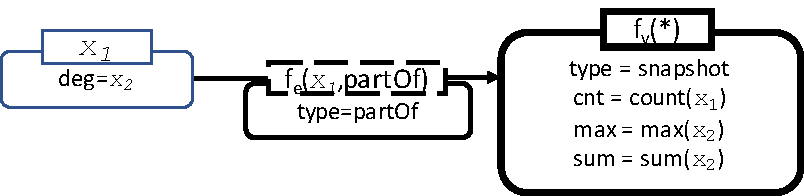
\includegraphics[width=3.3in]{figs/snapshotncr.pdf}
\vspace{-0.4cm}
\caption{Navigational graph pattern $p_2$.}
\label{fig:snapshotncr}
\vspace{-0.2cm}
\end{figure}

\begin{enumerate}[itemindent=\dimexpr\labelwidth+\labelsep\relax,leftmargin=0pt]
\item Compute a temporally aggregated view of the graph into windows
  using the window-based node creation operator with \insql{always}
  node and edge quantifiers:

$\ttt_1 = \insql{node}^T_w(\mathsf{w=2~mon},\mathsf{r_v=always},\mathsf{r_e=always},wikitalk)$

\item Compute in-degree of each node with the aggregation operator:  $\ttt_2 = \insql{agg}^T_{p_1}(\ttt_1)$

\item Group all nodes that are present at a given time into a
  single node with the attribute-based node creation operator, using
  pattern $p_2$ in Figure~\ref{fig:snapshotncr}.  Accumulate max,
  sum, and count of \insql{deg} as properties at that
  node:  $\ttt_3 =\insql{node}^T_a(p_2,\ttt_2)$

%\item Keep only the new nodes using the vertex-subgraph operator.
%
%$\ttt_4 = \subv{p_3}{\ttt_3}$

\item Compute degree centrality at each time point using the vertex-map operator:  $\medmuskip=0mu\ttt_4 = \vmap{\mathsf{f_v=cent=(max*cnt-sum)/(cnt^2-3*cnt+2)}, \ttt_3}$
\end{enumerate}

%\subsection{Communities over Time} 
%
\eat{
Interaction networks are sparse because edges are so short-lived.  It
may be useful to zoom out in time by changing the time granularity of
the data such that all durations are, for example, in months or years.
This way more items are concurrent and the overall network is more
connected.  We call this kind of zooming out a change in temporal
resolution of the graph and we can use it as part of exploratory
analysis.  After decreasing temporal resolution we can run a community
detection algorithm, e.g., compute the connected components of the
network, and then consider the number of and size of connected
components.  
}
\eat{
To see whether communities form and at what time scale, we vary the
time scale and compute communities, e.g., through connected components
detection, group the nodes by the community they form and calculate
their size.  We can filter out nodes that represent communities
below a reasonable threshold, for example of size smaller than two:
}
\eat{
\begin{figure}
\centering
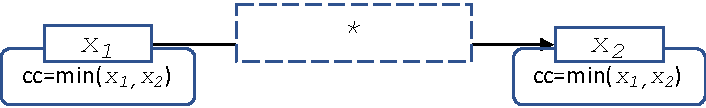
\includegraphics[width=3in]{figs/ccp.pdf}
\vspace{-0.2cm}
\caption{Connected components pattern $p_3$.}
\vspace{-0.2cm}
\label{fig:ccp}
\end{figure}
}
\eat{
\begin{enumerate}[itemindent=\dimexpr\labelwidth+\labelsep\relax,leftmargin=0pt]
\item Aggregate the graph into 6-month windows:
}
%$\ttt_1 = \insql{node}^T_w(\mathsf{w=6~mon},\mathsf{r_v=always},\mathsf{r_e=always},wikitalk)$
%
%\item Compute weakly connected components at each time point using the aggregation operator and a pattern $p_3$ depicted in Figure~\ref{fig:ccp}:  $\ttt_2 = \insql{agg}^T_{p_3}(\ttt_1)$
%$\ttt_2 = \insql{pregel}^T_{cc} (\mathsf{pname=comp}, \ttt_1)$
%
%\item Add a node for each connected component, and compute the size of
%  the connected component, using attribute-based node creation and
%  pattern $p_4$ (not depicted): 
%
%$\ttt_3 =  \insql{node}^T_a(p_4,\ttt_2)$
%
%\item Filter out nodes that represent communities too small to be
%  useful (e.g., of 1-2 people) using vertex-subgraph and a simple
%  pattern $p_5$ with \insql{size>3} predicate (not depicted): 
%
%$\ttt_4 = \sub{p_5}{\ttt_3}$
%\end{enumerate}

\subsection{ Spread of Information} 

We can analyze evolving interaction networks to study how information
spreads over time.  Suppose each edge has a \insql{topic} attribute
that indicates what each communication between users is about.  To see
how far and how quickly information spreads, we can compute {\em
  journeys}.  A journey connects any two nodes by a new edge if there
is a path between them such that the edge times are non-decreasing.
For example, a journey can be over edges that all co-exist or over
edges that follow each other in time.  In this example, we connect any
two nodes that have a path between them on the same topic and assign
new edges a length property equal to the sum of the edges in the path.
This is an example of an edge creation operation extended for evolving
graphs.  To see how far information may travel and who the sources
are, we can select a subset of the network, consisting only of nodes
that originate the longest edges.

\begin{figure}
\centering
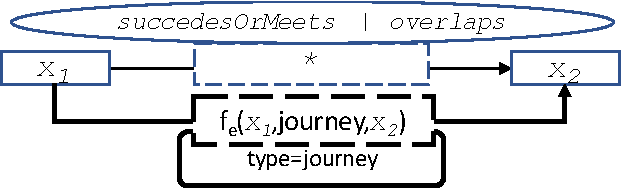
\includegraphics[width=2.5in]{figs/journeys.pdf}
\vspace{-0.2cm}
\caption{A journey pattern $p_7$.}
\label{fig:journeysp}
\vspace{-0.2cm}
\end{figure}

\begin{enumerate}[itemindent=\dimexpr\labelwidth+\labelsep\relax,leftmargin=0pt]
\item Select only the portion of the graph that relates to the topic
  of interest using the subgraph operator and a pattern with
  \insql{topic = 'Hurricane Sandy'} pattern (not depicted):

$\ttt_1 = \sub{p_6}{wikitalk}$

\item Connect every pair of nodes that has a path between them with non-decreasing time periods using the edge creation operator using pattern $p_7$ in Figure~\ref{fig:journeysp}:

$\ttt_2 = \insql{edge}^T_{p_7}(\ttt_1,\ttt_1)$

\eat{For readability, the TNGP in this query, expressed as a set of
Datalog rules, where $f$ is a Skolem function, is:
}
%\begin{small}
%\begin{verbatim}
%teprime(e,x,y,a,p) <- te1(e,x,y,_,p),a.length=1
%teprime(f(x,z,a),x,z,a,p) <- teprime(_,x,y,a1,p1), te1(_,y,z,a2,p2),
%                             a.length=a1.length+z2.length, p1<p2
%\end{verbatim}
%\end{small}}

\item Select the node with the largest number of edges using the vertex-subgraph operator and a pattern with \insql{max(sum(x))} expression (not depicted):

$\ttt_3 = \sub{p_8}{\ttt_2}$
\end{enumerate}
